% CODIGO DE ORDENACIONES
\definecolor{lightergray}{RGB}{247,247,247}
\definecolor{darkgreen}{RGB}{36,135,20}
\definecolor{green_comment}{RGB}{0,128,0}
\definecolor{redcell}{RGB}{238,176,176}
\definecolor{greencell}{RGB}{217,234,211}



\chapter{Estudio empírico}

Después de implementar y diseñar los algoritmos y mejoras utilizando MPI, llevamos a  cabo un análisis exhaustivo para evaluar los tiempos de ejecución, realizar pruebas, contrastar resultados y extraer conclusiones.

Primero se ejecutan distintas pruebas en un ordenador normal, para luego ejecutar las mejores implementaciones en un cluster con varios ordenadores y muchos procesos.



\begin{tcolorbox}[boxrule=0.5pt, fontupper=\small]
\scriptsize
\textcolor{red}{
Ordenador básico: 8 núcleos, 16 procesos lógicos y 32gb de ram\\
\\
\\
\\
Cluster:
\\
}
\end{tcolorbox}
	



% ------------------------------------------------------------------------------------------------
% --- ORDENACIONES  ------------------------------------------------------------------------------
% ------------------------------------------------------------------------------------------------


% VARIABLES Y PRUEBAS DE ORDENACIONES 
\begin{flushleft}
\textbf{Ordenaciones}
\begin{mdframed}[roundcorner=5pt]
\textbf{\underline{Pruebas}}
\vspace{0.1cm}

\scriptsize	
\textbf{Arrays de enteros, siempre en el caso peor,} es decir, ordenados de forma \textbf{decreciente}, por lo que tiene que ejecutar el mayor número de comparaciones para ordenarlo de forma creciente.\\	
Las pruebas se ejecutan sobre el mismo array de enteros, y se van aumentando el tamaño para medir los tiempos de ejecución. En cada prueba se añaden \textit{x} elementos más a ordenar.
\begin{tcolorbox}[boxrule=0.5pt, fontupper=\small]
	\scriptsize
	El incremento del tamaño viene dado de la siguiente forma:\\
	- [20-1.000) $\rightarrow$ 20 elementos.\\
	- [1.000-10.000) $\rightarrow$ 250 elementos.\\
	- [10.000-100.000) $\rightarrow$ 1.000 elementos.\\
	Para MergeSort, al ser un algoritmo mas eficiente, no se añade de mil en mil al llegar a 10.000 elementos, se mantiene el incremento de 250 elementos.

\end{tcolorbox}

\end{mdframed}
\end{flushleft}

\newpage

\begin{figure}[h]
	\centering
	\begin{tikzpicture}
		\begin{axis}[
			xlabel={Tam. Array ($10^4$)},
			ylabel={Tiempo (s)},
			legend pos=north west,
			grid=major,
			width=0.70\textwidth,
			height=0.4\textwidth
			]
			
			% Plot data from the file without markers, with different colors, and thicker lines
			\addplot [mark=none, color=red, line width=1.2pt] table [x index=0, y index=1, col sep=space] {files/sortn2.txt};
			\addplot [mark=none, color=blue, line width=1.2pt] table [x index=0, y index=2, col sep=space] {files/sortn2.txt};
			\addplot [mark=none, color=darkgreen, line width=1.2pt] table [x index=0, y index=3, col sep=space] {files/sortn2.txt};
			\addplot [mark=none, color=green, line width=1.2pt] table [x index=0, y index=4, col sep=space] {files/sortn2.txt};
			\addplot [mark=none, color=black, line width=1.2pt] table [x index=0, y index=5, col sep=space] {files/sortn2.txt};
			
			% Add legends
			\addlegendentry{BubbleSort}
			\addlegendentry{InsertionSort}
			\addlegendentry{SelectionSort}
			\addlegendentry{SequentialSort }
			\addlegendentry{SequentialSort\_MPI(5)}
			
		\end{axis}
	\end{tikzpicture}
	\caption{Tiempo de ejecución de los algoritmos de ordenación cuadráticos}
\end{figure}

La implementación aplicando MPI sobre SequentialSort tiene un speed-up proporcional al número de procesos ejecutándose al llegar a un cierto número de elementos a ordenar.  %TODO
Al paralelizar el trabajo de SequentialSort, se pueden obtener mejores resultados que SelectionSort al usar cinco o más procesos workers.

De las ordenaciones básicas con coste cuadrático (O(N2)) comentadas anteriormente, SelectionSort es la que mejores resultados obtiene, y BubbleSort la peor, siendo aproximadamente 3.5 veces más lenta con 70.000 elementos. 
La ordenación diseñada SequentialSort es incluso más rápida que dos de las más famosas, debido a la simpleza de las operaciones aplicadas en la ordenación. Esta ordenación hace N2 comparaciones, pero al no modificar elementos del array sigue siendo más rápida que las otras.


%\lstset{language=python, 
%	breaklines=true, 
%	basicstyle=\footnotesize,
%	backgroundcolor=\color{lightergray}}	
%\begin{lstlisting}[frame=single]
%	def selection_sort(a):			def sequential_sort(a):
%	n = len(a)				  INF=sys.maxsize
%	minE = 0				  n=len(a)
%	pos = 0			  	  b=[(INF) for i in range(n)]  
%	
%	for i in range(n-1):			  for i in range(n):
%	minE = a[i]			    cont=0
%	pos = i				    val=a[i]
%	for j in range(i+1, n):		    for i in range(n):  
%	if minE > a[j]:		      if a[i]<val: cont+=1
%	minE = a[j]				while b[cont]!=INF: 
%	pos = j				  cont+=1
%	b[cont]=val
%	tmp = a[i]
%	a[i] = a[pos]
%	a[pos] = tmp
%	
%\end{lstlisting}

%Sequential sort + Uso de memoria
\begin{figure}[h!]
	\centering
	\begin{tikzpicture}
		\begin{groupplot}[group style={
				group size=2 by 1,
				horizontal sep=1.5cm, % Adjust horizontal separation between plots
				vertical sep=0.5cm}, % Adjust vertical separation between plots           
			grid=major,
			width=0.45\textwidth, height=0.30\textwidth, % Adjust size as needed      
			tick label style={font=\tiny} % Adjust font size of tick labels  
			]
			
			% First plot
			\nextgroupplot[
			title={}, 
			ylabel=Tiempo \tiny de ejecución (s), 
			xlabel=Tam. Array,
			legend pos=north west
			]
			\addplot [mark=none, color=red, line width=1.2pt] table [x index=0, y index=1, col sep=space] {files/sequential.txt};
			\addplot [mark=none, color=black, line width=1.2pt] table [x index=0, y index=2, col sep=space] {files/sequential.txt};
			\addplot [mark=none, color=darkgreen, line width=1.2pt] table [x index=0, y index=3, col sep=space] {files/sequential.txt};
			
			% Add legends
			\addlegendentry{Básico}
			\addlegendentry{MPI\_1}
			\addlegendentry{MPI\_2}
			
			% Second plot
			\nextgroupplot[
			title={},
			xtick={2,3,4,5,6,7,8,9,10}, % Adjust x-tick positions as needed
			ytick={0,2,4,6,8,10,12}, % Adjust y-tick positions as needed
			legend pos=north west,			
			xlabel=Num. Procesadores,
			ylabel=Memoria \tiny(Copias del array)
			]
			\addplot[name path=blue, color=blue, mark=square] table {files/sequentialMem.txt};
			\addlegendentry{MPI\_1}
			
			\addplot[name path=orange, color=orange, mark=triangle] table [y index=2] {files/sequentialMem.txt};
			\addlegendentry{MPI\_2}
			
			\addplot [color=blue!50, fill=blue!50, fill opacity=0.3] fill between [of=blue and orange, soft clip={domain=2:10}];
			
			\addplot [name path=axis, draw=none] coordinates {(2,0) (10,0) };	
			
			\addplot [color=orange!50, fill=orange!50, fill opacity=0.3] fill between [of=orange and axis, soft clip={domain=2:10}];
			
		\end{groupplot}  
		
	\end{tikzpicture}
	\caption{Mejoras MPI SequentialSort + Memoria}
\end{figure}
\newpage

La primera mejora es un poco más eficiente pero consume mucho más memoria que la segunda. En cuestión de complejidad temporal es un poco mejor repartir el array entero entre los workers, pero la complejidad espacial para esta implementación aumenta de manera lineal en proporción al número de procesadores. Por lo que teniendo en cuenta ambos aspectos es mejor la segunda implementación, dividir el array entre los workers y recibir elementos para comprobar su posición ordenada.\\


MergeSort tiene un coste temporal de O(NlogN), y al aplicar la mejora comentada se puede apreciar una notoria reducción del tiempo de ejecución, llegando a tener un speedup aproximado de 15.5 usando dieciséis workers, casi el speedup ideal. Es cierto que se podrían aplicar otras técnicas para reducir mucho más el tiempo, pero quería demostrar que en la computación de alto rendimiento se pueden obtener buenos resultados con estrategias no tan efectivas pero bien paralelizadas.


% HISTOGRAMA CON VARIOS PROCESOS
\begin{figure}[h!]
\begin{tikzpicture}
	\begin{axis}[
		ybar,
		bar width=0.35cm,
		ylabel={Tiempo de ejecución (s)},
		xlabel={Tamaño del array (miles de elementos)},
		symbolic x coords={25, 50, 75, 100},
		xtick=data,
		enlarge x limits=0.2,
		ymin=0,
		%width=15cm,
		%height=10cm,
		width=\textwidth,
		height=0.45\textwidth,
		legend style={at={(0.5,-0.15)}, anchor=north, legend columns=-1},
		area legend
		]
		
		\addplot+[ybar, pattern=vertical lines, draw=black] plot coordinates 
		{(25, 1.12) (50, 4.39) (75, 10.0) (100, 21)};
		\addplot+[ybar, pattern=grid, draw=black] plot coordinates 
		{(25, 0.67) (50, 2.58) (75, 5.70) (100, 10.15) };
		\addplot+[ybar, pattern=dots, draw=black] plot coordinates 
		{(25, 0.23) (50, 0.93) (75, 2.09) (100, 3.35) };
		\addplot+[ybar, pattern=crosshatch, draw=black] plot coordinates 
		{(25, 0.09) (50, 0.34) (75, 0.72) (100, 1.39)};
		\addplot+[ybar, pattern=checkerboard, draw=black] plot coordinates 
		{(25, 0.059) (50, 0.18) (75, 0.41) (100, 0.71)};
		
		
		\legend{Secuencial, MPI(4),MPI(8),MPI(16),MPI(32)}
	\end{axis}	
\end{tikzpicture}
\caption{Tiempo de ejecución MPI MergeSort}
\end{figure}


Con dos workers ejecutándose no reduce el tiempo de ejecución, lo duplica. Al aplicar ordenaciones cuadráticas y solo tener dos workers, el cómputo es igual que aplicar una ordenación cuadrática con la mitad del array original.

La memoria está optimizada puesto que el master se encarga de dividir eficientemente el array entero entre todos los workers, teniendo solo dos copias del array, la que tiene el master y la otra dividida entre los procesos que se encargan de ordenarlo. Al terminar un proceso con la sincronización en mariposa, se termina la ejecución del proceso liberando memoria una vez ha enviado al proceso correspondiente su subarray ordenado.


\color{blue} TODO CLUSTER

\color{black}
\newpage

% ------------------------------------------------------------------------------------------------
% --- MATRIZ -------------------------------------------------------------------------------------
% ------------------------------------------------------------------------------------------------
% TODO MATRIZ

\begin{flushleft}
	\textbf{Matriz}
\end{flushleft}

\color{blue} TODO...

\color{black}


\newpage
% ------------------------------------------------------------------------------------------------
% --- JERARQUICO AGLOMERATIVO --------------------------------------------------------------------
% ------------------------------------------------------------------------------------------------


\begin{flushleft}
\textbf{Algoritmos de Agrupación}
	\begin{mdframed}[roundcorner=5pt]
		\textbf{\underline{Pruebas}}
		\vspace{0.1cm}
		
		\scriptsize	
		\textbf{Las poblaciones que se usan en cada algoritmo se han generado previamente de manera aleatoria}, delimitando un intervalo [-10, 10] para todas las dimensiones disponibles. Para crear los gráficos se ejecutó muchas veces con diferentes tamaños para guardar los tiempos de ejecución con poblaciones de diferentes tamaños. Se añaden \textit{x} elementos a las poblaciones.
		
		
		\begin{tcolorbox}[boxrule=0.5pt, fontupper=\small]
			\scriptsize
			Para las implementaciones de K-Medias y Jerárquico Aglomerativo se aplican el mismo incremento que en las ordenaciones:
			El incremento del tamaño viene dado de la siguiente forma:\\
			- [20-1.000) $\rightarrow$ 20 elementos.\\
			- [1.000-10.000) $\rightarrow$ 250 elementos.\\
			- [10.000-100.000) $\rightarrow$ 1.000 elementos.\\
			
			Para K-Vecinos más cercanos (KNN), al ser un algoritmo lineal, se guarda el tiempo de ejecución cada veinte nuevos individuos categorizados.
			
		\end{tcolorbox}
		
	\end{mdframed}
\end{flushleft}


\textbf{Jerárquico Aglomerativo:}

Cuando la complejidad del cálculo de las distancias entre clusters es constante (aplicando centroide), el tiempo de ejecución no varía al usar un determinado tipo de distancia.
No obstante, cuando se aplican distancias entre clusters con coste cuadrático (enlace simple o completo), la distancia euclídea tarda más, porque para realizar el cálculo, usa potencias y raíces cuadradas.



% JERARQUICO AGLOMERATIVO (EUCLIDEA y MANHATTAN)
\begin{figure}[!h]
	\centering
	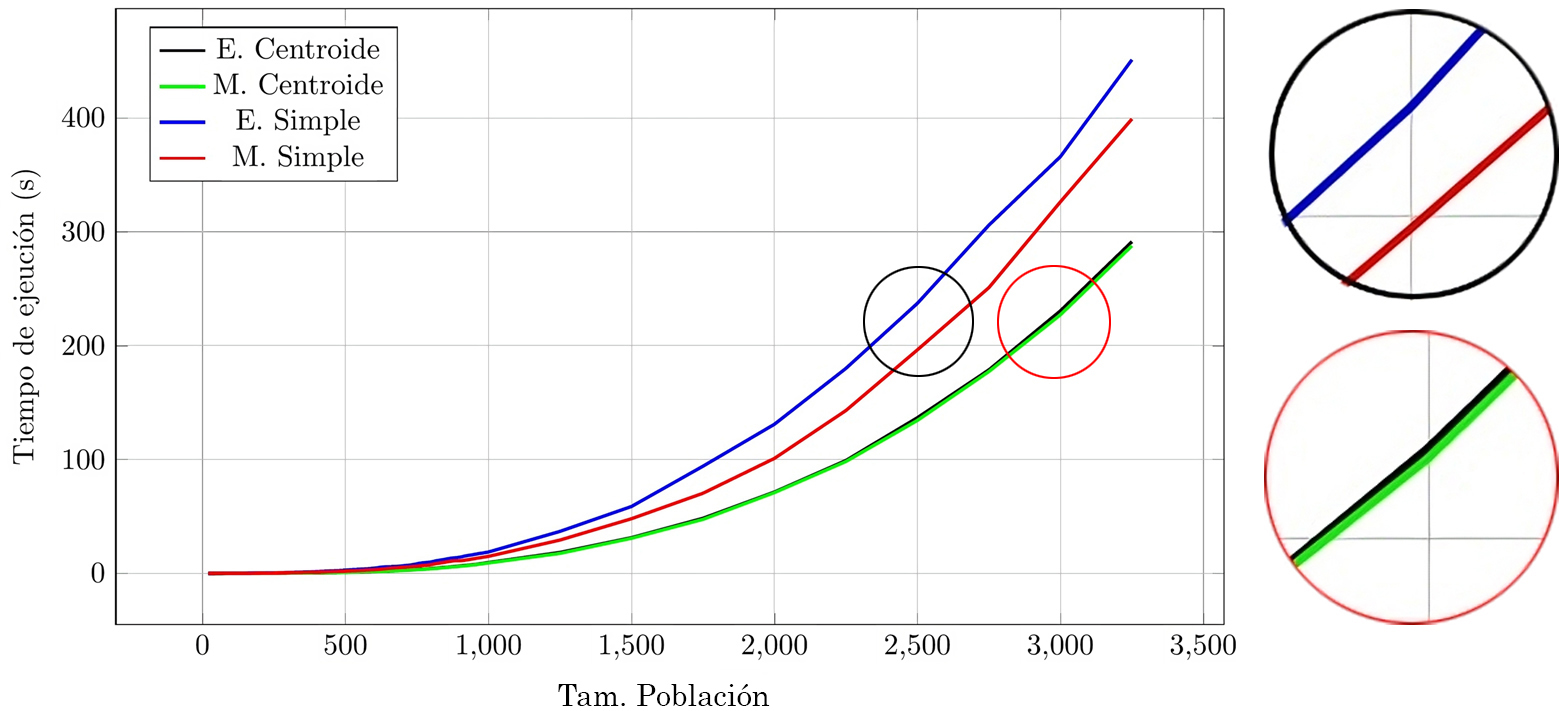
\includegraphics[width=0.8\textwidth]{images/chapter_4/jerarquico}
	\caption{Tiempo de ejecución del algoritmo básico Jerarquíco Aglomerativo}
	\label{fig:prueba_jerarquicosec}
\end{figure}

Al principio no hay tanta diferencia, pero conforme se aumenta la población, los tiempos de ejecución empiezan a distinguirse. El tiempo de ejecución para calcular la distancia entre dos clusters depende del número de individuos de los mismos, y conforme se aumenta la población aumenta el número de repeticiones del cálculo de las distancias, además de aumentar los individuos en cada cluster lo que también perjudica al tiempo de ejecución.


Distancia entre clusters por \textbf{centroide}.
La segunda mejora de dividir entre los workers el cálculo de distancias, no se puede aplicar. Debido a que el cálculo de distancias es constante, no surte mucho efecto dividir la fila que se tiene que recalcular, porque el coste total es lineal. Pero la mejora principal reduce considerablemente el tiempo de ejecución.




% JERARQUICO AGLOMERATIVO: HISTOGRAMA CON VARIOS PROCESOS
\begin{figure}[!h]
	\centering
	\begin{tikzpicture}
		\begin{axis}[
			ybar,
			bar width=0.35cm,
			ylabel={Tiempo de ejecución (s)},
			xlabel={Tam. Array},
			symbolic x coords={1000, 2500, 5000},
			xtick=data,
			enlarge x limits=0.2,
			ymin=0,
			width=\textwidth,
			height=0.45\textwidth,
			legend style={at={(0.5,-0.15)}, anchor=north, legend columns=-1},
			area legend
			]
			
			\addplot+[ybar, pattern=vertical lines, draw=black] plot coordinates 
			{(1000, 7.61) (2500, 141.59) (5000, 1098.29)};
			\addplot+[ybar, pattern=grid, draw=black] plot coordinates 
			{(1000, 4.81) (2500, 79.61) (5000, 617.44)};
			\addplot+[ybar, pattern=dots, draw=black] plot coordinates 
			{(1000, 2.75) (2500, 47.36) (5000, 379.42) };
			\addplot+[ybar, pattern=crosshatch, draw=black] plot coordinates 
			{(1000, 2.24) (2500, 38.55) (5000, 304.12) };
			\addplot+[ybar, pattern=checkerboard, draw=black] plot coordinates 
			{(1000, 1.98) (2500, 33.13) (5000, 260.77)};
			
			
			\legend{Secuencial, MPI(2),MPI(4),MPI(6),MPI(8)}
		\end{axis}
	\end{tikzpicture}
	\caption{ MPI Jerarquico Aglomerativo, Dist. por centroide}
\end{figure}

% TODO Jerarquico Aglom, Dist. Simple 

\color{blue} TODO PRUEBAS D. SIMPLE/COMPLETO ...
% TODO Jerarquico Aglom CLUSTER
TODO CLUSTER

\color{black}


\newpage
% ------------------------------------------------------------------------------------------------
% --- KMEDIAS ------------------------------------------------------------------------------------
% ------------------------------------------------------------------------------------------------
\textbf{K-MEDIAS}

El algoritmo anterior no tiene ninguna variable que modifique el tiempo de ejecución. Sin contar la distancia entre clusters. Esta técnica de agrupación tiene un coste temporal mucho menor que el aglomerativo, \textit{O(N*K*iter)} siendo N el tamaño de la población, iter las iteraciones  hasta que no cambien los centros. \textit{(N $\gg$ K,iter)} K e iter no son valores muy altos por lo que la complejidad no llega a ser cuadrática.

Para las pruebas realizadas se usa un valor K=10, y se usan cuatro procesos workers para la mejora MPI:


\begin{figure}[!h]
	\centering
	\begin{tikzpicture}
		\begin{axis}[
			xlabel={Tam. Población ($10^5$)},
			ylabel={Tiempo de ejeución (s)},
			legend pos=north west,
			grid=major,
			width=\textwidth,
			height=0.4\textwidth
			]
			
			% Plot data from the file without markers, with different colors, and thicker lines
			\addplot [mark=none, color=blue, line width=1.2pt] table [x index=0, y index=1, col sep=space] {files/kmedias.txt};
			\addplot [mark=none, color=red, line width=1.2pt] table [x index=0, y index=2, col sep=space] {files/kmedias.txt};
			\addplot [mark=none, color=darkgreen, line width=1.2pt] table [x index=0, y index=3, col sep=space] {files/kmedias.txt};
			\addplot [mark=none, color=black, line width=1.2pt] table [x index=0, y index=4, col sep=space] {files/kmedias.txt};
			
			
			% Add legends
			\addlegendentry{Euclidea}
			\addlegendentry{Manhattan}
			\addlegendentry{Euclidea\_MPI}
			\addlegendentry{Manhattan\_MPI}
			
			
		\end{axis}
	\end{tikzpicture}
	\caption{Tiempo de ejecución de KMedias}
\end{figure}


A medida que la población crece, los centros varían, debido a la inclusión de más individuos en el cálculo de las nuevas posiciones de los centros, provocando una variación en el número de iteraciones del algoritmo para que los centros no cambien. 
El tiempo de ejecución no aumenta en proporción al tamaño, si no que varía dependiendo de la composición de los individuos y por eso hay tantos picos. El aumento de la población no necesariamente implica una ejecución más lenta en comparación con una población menor.
Las mejoras MPI, son bastante buenas. Haciendo el mismo número de iteraciones que las implementaciones secuenciales, no hay picos muy pronunciados. Lo más seguro es que al aumentar la población se empiecen a pronunciar.





\begin{figure}[!h]
	\centering
	\begin{tikzpicture}
		\begin{axis}[
			xlabel={Tam. Población},
			ylabel={SpeedUp},
			legend pos=north east,
			grid=major,
			width=0.85\textwidth,
			height=0.40\textwidth
			]
			
			% Plot data from the file without markers, with different colors, and thicker lines
			\addplot [mark=none, color=darkgreen, line width=1.7pt] table [x index=0, y index=1, col sep=space] {files/kmedias_speedup.txt};
			\addplot [mark=none, color=red, line width=0.3pt] table [x index=0, y index=2, col sep=space] {files/kmedias_speedup.txt};
			\addplot [mark=none, color=blue, line width=0.3pt] table [x index=0, y index=3, col sep=space] {files/kmedias_speedup.txt};
			
			
			% Add legends
			\addlegendentry{Ideal}
			\addlegendentry{Euclidea}
			\addlegendentry{Manhttan}
			
			
		\end{axis}
	\end{tikzpicture}
	\caption{SpeedUp - KMedias}
\end{figure}

El speedup es muy curioso. A partir de diez mil individuos de población, el speedup es aproximadamente el ideal para ambas distancias, contando solo que los workers son los que trabajan y el master solo recibe la asignación y calcula los nuevos centros. Pero lo curioso es que con la población generada aleatoria, y un tamaño relativamente pequeño llega a duplicar el speedup ideal. Lo primero que se puede venir a la mente es que hace menos iteraciones, pero esto no es así, puesto que ejecuta el mismo número de iteraciones en ambas implementaciones. 

% TODO ¿Poner gráfico con el número de iteraciones para cada tamaño? Serían 2 líneas iguales.



% KMEDIAS: HISTOGRAMA CON VARIOS PROCESOS
\begin{figure}[!h]
	\centering
	\begin{tikzpicture}
		\begin{axis}[
			width=0.85\textwidth,
			height=0.40\textwidth,
			ybar,
			bar width=0.35cm,
			ylabel={Tiempo de ejecución (s)},
			xlabel={Tam. de la Población},
			symbolic x coords={25000, 50000, 75000, 100000},
			xtick=data,
			enlarge x limits=0.2,
			ymin=0,
			legend style={at={(0.5,-0.15)}, anchor=north, legend columns=-1},
			area legend,
			legend columns=4,
			]
			
			% Histo
			\addplot+[ybar, pattern=vertical lines, draw=black] plot coordinates 
			{(25000, 0.62) (50000, 1.31) (75000, 1.66) (100000, 2.56)};				
			\addplot+[ybar, pattern=grid, draw=black] plot coordinates 
			{(25000, 1.69) (50000, 4.22) (75000, 5.19)  (100000, 8.76)};						
			\addplot+[ybar, pattern=dots, draw=black] plot coordinates 
			{(25000, 8.29) (50000, 33.80) (75000, 79.83) (100000, 79.56)};						
			\addplot+[ybar, pattern=crosshatch, draw=black] plot coordinates 
			{(25000, 19.93) (50000, 56.03) (75000, 109.96) (100000, 123.16)};
			
			\addplot[smooth, mark=diamond, green] plot coordinates
			{(25000, 0.62) (50000, 1.31) (75000, 1.66) (100000, 2.56)};
			\addplot[smooth, mark=diamond, blue] plot coordinates
			{(25000, 1.69) (50000, 4.22) (75000, 5.19)  (100000, 8.76)};
			\addplot[smooth, mark=diamond, black] plot coordinates
			{(25000, 8.29) (50000, 33.80) (75000, 79.83) (100000, 79.56)};
			\addplot[smooth, mark=diamond, red] plot coordinates
			{(25000, 19.93) (50000, 56.03) (75000, 109.96) (100000, 123.16)};
			
			\legend{5, 10, 25, 50}
		\end{axis}
	\end{tikzpicture}
	\caption{KMedias variando K}
\end{figure}

% TODO KMedias CLUSTER

\color{blue} TODO CLUSTER

\color{black}

\newpage
% ------------------------------------------------------------------------------------------------
% --- KNN ----------------------------------------------------------------------------------------
% ------------------------------------------------------------------------------------------------

\textbf{KNN}

En cada iteración de este algoritmo de aprendizaje supervisado, usa una población categorizada para agrupar un único individuo, no como en los anteriores que tiene que terminar todas las iteraciones para agrupar toda una población.

Para las pruebas realizadas se usa un valor de K=15, impar para que no pueda existir empates. Hay dos formas de realizar la agrupación. Si se actualiza la población conforme se categorizan los individuos nuevos, la población final será mucho más precisa que si no se actualiza, pero tardará más tiempo en ejecutarse. 


% KNN BASICO
\begin{figure}[h!]
	\centering
	\begin{tikzpicture}
		\begin{axis}[
			xlabel={Tam. Población ($10^5$)},
			ylabel={Tiempo de ejeución (s)},
			legend pos=north west,
			legend columns=2,
			grid=major,
			width=\textwidth,
			height=0.45\textwidth
			]
			
			% Plot data from the file without markers, with different colors, and thicker lines
			\addplot [mark=none, color=darkgreen, line width=1.2pt] table [x index=0, y index=1, col sep=space] {files/knn.txt};
			\addplot [mark=none, color=red, line width=1.2pt] table [x index=0, y index=3, col sep=space] {files/knn.txt};
			\addplot [mark=none, color=black, line width=1.2pt] table [x index=0, y index=2, col sep=space] {files/knn.txt};
			
			\addplot [mark=none, color=blue, line width=1.2pt] table [x index=0, y index=4, col sep=space] {files/knn.txt};
			
			
			% Add legends
			\addlegendentry{Euclidea}
			\addlegendentry{Euclidea\_Act}
			\addlegendentry{Manhattan}
			
			\addlegendentry{Manhattan\_Act}
			
			
		\end{axis}
	\end{tikzpicture}
	\caption{Tiempo de ejecución para KNN}
\end{figure}

Cuando la población se actualiza, aumenta el tiempo de ejecución, y se puede apreciar la diferencia entre los tipos de distancia. A largo plazo la distancia Euclídea tardará mucho más que la Manhattan, por tener una complejidad de cálculo mayor. 
Cuando la población es constante, los tiempos de ejecución aumentan con el tamaño de la población a predecir de forma lineal, y el uso de distancias no afecta casi al rendimiento.


% TODO MEJORAR CALIDAD
\begin{figure}[!h]
	\centering
	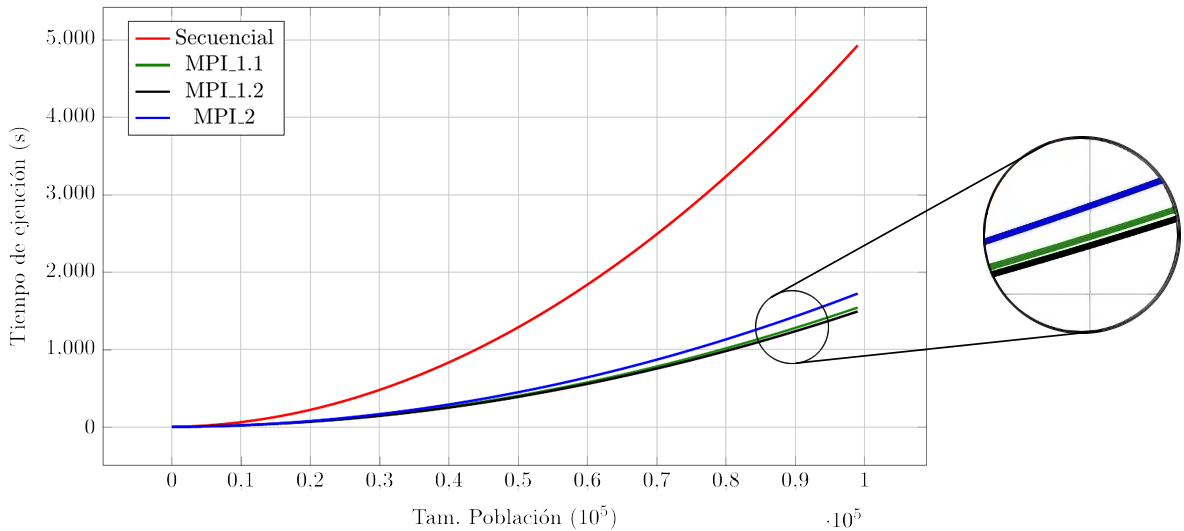
\includegraphics[width=0.8\textwidth]{images/chapter_4/knn_mpi}
	\caption{Tiempo de ejecución del algoritmo básico Jerarquíco Aglomerativo}
	\label{fig:example}
\end{figure}

Las dos implementaciones son aproximadamente iguales, siendo mejor la segunda implementación de la primera mejora. Añadir los individuos categorizados de la iteración anterior cuando cada worker finaliza la búsqueda de los K vecinos más cercanos en la iteración actual, elimina el tiempo de espera que tenía la primera implementación, reduciendo levemente el tiempo.
La segunda mejora, además de ser levemente peor en cuestión de complejidad temporal, es mucho peor en complejidad espacial. Dividir la población a predecir conlleva un mayor consumo de memoria, al tener que tener la población entera en cada proceso. En la primera mejora se reparten equitativamente los individuos nuevos, es decir, en cada iteración el master envía a un único proceso el individuo categorizado.


1. La primera mejora acaba con dos copias de la población inicial y predicha (una en el master y la otra repartida entre los procesos). 
2. La segunda mejora acaba con N copias, siendo N el número de procesos ejecutados.


\vspace{0.1cm}

\begin{figure} [!h]
	\centering
	\begin{tikzpicture}
		\begin{axis}[
			xlabel={Tam. Población},
			ylabel={SpeedUp},
			legend pos=south east,			
			legend columns=3,
			grid=major,
			width=0.85\textwidth,
			height=0.35\textwidth
			]
			
			% Plot data from the file without markers, with different colors, and thicker lines
			\addplot [mark=none, color=darkgreen, line width=0.8pt] table [x index=0, y index=1, col sep=space] {files/knn_speedup.txt};
			\addplot [mark=none, color=red, line width=0.8pt] table [x index=0, y index=2, col sep=space] {files/knn_speedup.txt};
			\addplot [mark=none, color=blue, line width=0.8pt] table [x index=0, y index=3, col sep=space] {files/knn_speedup.txt};
			
			
			% Add legends
			\addlegendentry{Ideal}
			\addlegendentry{MPI\_1}
			\addlegendentry{MPI\_2}
			
			
		\end{axis}
	\end{tikzpicture}
	\caption{SpeedUp - KNN}
\end{figure}

Al principio es mejor dividir la poblacion a predecir, pero a largo plazo es más efectivo dividir la poblacion categorizada, además de tener menos complejidad espacial.



% TODO KNN SIN ACTUALIZAR? 

\vspace{1cm}

\color{blue} TODO ? Añadir un estudio del algoritmo sin actualizar? Así a lo mejor se puede comprobar que es mejor la segunda implementación cuando las poblaciones no cambian.

% TODO KNN CLUSTER
TODO CLUSTER
\color{black}

\newpage


% ------------------------------------------------------------------------------------------------
% --- RL -----------------------------------------------------------------------------------------
% ------------------------------------------------------------------------------------------------

\textbf{RL}

Una vez implementada este preprocesado y comparándolo con el sin procesar, los resultados son parecidos. Pero con en la búsqueda de los mejores hiper parámetros, da mejores resultados al preprocesar. No hace acciones innecesarias y le permite explorar mejor el entorno y no entrar en bucles.

Estas pruebas se realizan con tres distintos laberintos, ejecutando varias veces para hacer un cálculo más eficaz del tiempo de ejecución para cada laberinto. Las matrices son cuadradas, y se generan de manera aleatoria con \textit{30, 50 y 100 filas.}

\begin{figure}[!h]
	\centering
	\begin{tikzpicture}
		\begin{axis}[
			xlabel={Tam. del Laberinto},
			ylabel={Tiempo de ejeución (s)},
			legend pos=north west,
			grid=major,
			width=\textwidth,
			height=0.35\textwidth
			]
			
			% Plot data from the file without markers, with different colors, and thicker lines
			\addplot [mark=none, color=red, line width=1.2pt] table [x index=0, y index=1, col sep=space] {files/rl.txt};
			\addplot [mark=none, color=darkgreen, line width=1.2pt] table [x index=0, y index=2, col sep=space] {files/rl.txt};
			
			% Add legends
			\addlegendentry{Normal}
			\addlegendentry{Preprocesado}
			
			
		\end{axis}
	\end{tikzpicture}
	\caption{Tiempo de ejecución para RL}
\end{figure}


Para realizar la búsqueda mencionada se aplica la mejora de dividir el trabajo entre varios procesos. El master se encarga de mandar combinaciones a los workers. Dependiendo de la precisión, puede llegar a haber muchas por el poder de la combinatoria, y este proceso ser muy lento. El speedup es proporcional al número de nodos ejecutando combinaciones en paralelo.

Esta búsqueda es muy útil para encontrar configuraciones que funcionen en el entorno.
La mejora de matriz dividida no funciona correctamente, se queda en bucles en la mayoría de configuraciones que funcionan para la implementación secuencial del algoritmo. Con unos valores-Q previamente entrenados si funciona, pero la etapa de entrenamiento no funciona.

\newpage

% TODO RL 

\vspace{1cm}

\color{blue} TODO ? Añadir un estudio del algoritmo sin actualizar? Así a lo mejor se puede comprobar que es mejor la segunda implementación cuando las poblaciones no cambian.

% TODO RL CLUSTER
TODO CLUSTER
\color{black}
\newpage

% ------------------------------------------------------------------------------------------------
% --- PEV ----------------------------------------------------------------------------------------
% ------------------------------------------------------------------------------------------------



\begin{flushleft}
	\textbf{PEV}
	\begin{mdframed}[roundcorner=5pt]
		\textbf{\underline{Pruebas}}
		\vspace{0.1cm}
		
		\scriptsize		
		Para el algoritmo se ha aplicado un elitismo de 5\% conservando los mejores individuos de cada generación. Para el problema de árboles se aplica un método de control de bloating, para intentar reducir la alutra de los individuos. 		
		Para mejorar la aptitud de los individuos se aplica un desplazamiento, cuya finalidad es todos los individuos tengan valores positivos. Además de aplicar un escalado lineal, controlando la diversidad de las aptitudes.\\
			
		El método de evaluación depende del tipo de individuo. \\
		- Si es binario se calcula su valor real y se aplica una función matemática.  \\
		- Si es real, el problema del aeropuerto. \\
		- Si es árbol, el problema del cortacésped.\\
		
		Las pruebas realizadas para todas las gráficas se han ejecutado con las siguientes características:
		\begin{tcolorbox}[boxrule=0.5pt, fontupper=\small]
			\scriptsize
			Tam. Población = 100\\
			Núm. Generaciones = \{25,50,100,250,500,1000,2000\} \textbf{(Eje X)}\\
			Met. Selección: Torneo Determinístico, con un valor k=5.\\
			
			- Individuo Binario:\\
			Met. Cruce (p=0.6): Básica\\
			Met. Mutación (p=0.05): Básica \\
			P(x)=precision: \{P2: 30 bits, P10: 76 bits\}\\
			
			- Individuo Real:\\
			Met. Cruce (p=0.6): PMX\\
			Met. Mutación (p=0.3): Inserción \\
			AER(x)=aeropuerto: \{AER1: 10 vuelos, 3 pistas, AER1: 25 vuelos, 5 pistas, AER3: 100 vuelos, 10 pistas\}\\
			
			- Individuo Binario:\\
			Met. Cruce (p=0.6): Intercambio\\
			Met. Mutación (p=0.3): Terminal \\
			M(x)X(y)=matriz: \{M8X8: 8 filas, 8 columnas y 100 ticks; M100X100: 100 filas, 100 columnas y 10000 ticks\}
			
			
			
						
		\end{tcolorbox}
		
	\end{mdframed}
\end{flushleft}

Con las tres mejoras implementadas hay que tener en cuenta el tipo de individuo para cada problema, pues dependiendo del tipo, tardará más tiempo en determinadas funciones. Además de tener en cuenta el coste de la comunicación entre procesos.

Tiempo de ejecución (en segundos) de los métodos, para una operación. Es decir, el tiempo que tarda en inicializar, evaluar, seleccionar y mutar un único individuo, o cruzar dos individuos. 



% TODO CENTRAR TABLA
\begin{center}
	\begin{table}[!h]
	\centering
	\begin{tabular}{|c|c|c|c|c|c|c|}
		\hline
		\rowcolor{lightgray}
		\textbf{Datos} & \textbf{Funciones} & \textbf{Init(1)} & \textbf{Evaluación(1)} & \textbf{Selección(1)} & \textbf{Cruce(2)} & \textbf{Mutación(1)} \\
		\hline
		Precision: 2 & Binario & 2.56e-05 & 4.4e-06 & 8.56e-06 & \cellcolor{redcell} 1.36e-05 & \cellcolor{redcell} 1.53e-05 \\
		\hline
		Precision: 10 & Binario & 3.33e-05 & 5.44e-06 & 8.9e-06 & \cellcolor{redcell} 1.71e-05 & \cellcolor{redcell} 1.88e-05 \\
		\hline
		\makecell{aviones: 12 \\ pistas: 3} & Aeropuerto 1 & 7.04e-06 & \cellcolor{redcell} 2.55e-05 & 4.12e-06 & 1.48e-05 & 2.764e-06 \\
		\hline
		\makecell{aviones: 25 \\ pistas: 5} & Aeropuerto 2 & 1.36e-05 & \cellcolor{redcell} 6.55e-05 & 4.62e-06 & 2.4e-05 & 3.43e-06 \\
		\hline
		\makecell{aviones: 100 \\ pistas: 10} & Aeropuerto 3 & 3.97e-05 & \cellcolor{redcell} 4.3e-04 & 8.05e-06 & 4.18e-05 & 1.04e-05 \\
		\hline
		\makecell{M10x10 \\ ticks: 150} & Árbol & 6.12e-05 & \cellcolor{redcell} 6.47e-05 & 7.92e-05 & 2.33e-05 & 3.47e-07 \\
		\hline
		\makecell{M25x25 \\ ticks: 400} & Árbol & 6.16e-05 & \cellcolor{redcell} 1.65e-04 & 7.88e-05 & 2.32e-05 & 3.7e-07 \\
		\hline
		\makecell{M100x100 \\ ticks: 800} & Árbol & 6.41e-05 & \cellcolor{redcell} 3.66e-04 & 8.07e-05 & 2.09e-05 & 3.23e-07 \\
		\hline
	\end{tabular}
	\caption{PEV - Tiempos de cada método}
	\label{tab:sample}
	\end{table}
\end{center}

En rojo se marcan los métodos más tardíos para cada problema. 
Con individuos binarios, conviene dar más recursos a las operaciones de cruce y mutación. Y para los individuos reales y árboles la evaluación.






\begin{figure}[h!]
	\centering
	\begin{tikzpicture}
		\begin{groupplot}[
			group style={
				group size=3 by 1,
				horizontal sep=0.78cm,
				vertical sep=0.5cm},
			width=0.40\textwidth,
			height=0.40\textwidth,
			tick label style={font=\tiny} % Adjust font size of tick labels
			]
			
			% First plot
			\nextgroupplot[
			title={},
			ylabel= Tiempo de ejecución (s),
			legend style={at={(0.5,1.05)},anchor=south,legend columns=-1},
			xtick={25, 500, 1000, 1500, 2000} 
			]
			\addplot [mark=none, color=blue] table [x index=0, y index=1, col sep=space] {files/pev.txt};
			\addplot [mark=none, color=red] table [x index=0, y index=2, col sep=space] {files/pev.txt};
			\addlegendentry{\tiny P2}
			\addlegendentry{\tiny P10}
			
			% Second plot
			\nextgroupplot[
			title={},
			xlabel=Num. Generaciones,
			legend style={at={(0.5,1.05)},anchor=south,legend columns=-1},
			xtick={25, 500, 1000, 1500, 2000} 
			]
			\addplot [mark=none, color=blue] table [x index=0, y index=3, col sep=space] {files/pev.txt};
			\addplot [mark=none, color=green] table [x index=0, y index=4, col sep=space] {files/pev.txt};
			\addplot [mark=none, color=red] table [x index=0, y index=5, col sep=space] {files/pev.txt};
			\addlegendentry{\tiny AER 1}
			\addlegendentry{\tiny AER 2}
			\addlegendentry{\tiny AER 3}
			
			% Third plot
			\nextgroupplot[
			title={},
			legend style={at={(0.5,1.05)},anchor=south,legend columns=-1},
			xtick={25, 500, 1000, 1500, 2000} 
			]
			\addplot [mark=none, color=blue] table [x index=0, y index=6, col sep=space] {files/pev.txt};
			\addplot [mark=none, color=red] table [x index=0, y index=7, col sep=space] {files/pev.txt};
			\addlegendentry{\tiny M8X8}
			\addlegendentry{\tiny M100X10}
			
		\end{groupplot}        
	\end{tikzpicture}
	\caption{PEV Secuencial}
\end{figure}

% TODO PEV DESARROLLAR
Como solo varía el número de generaciones, las gráficas son lineales. Si se modifica de la misma forma el tamaño de la población, serían exponenciales, y tardarían mucho tiempo para ejecutarse.

1. El problema que aplica individuos binarios es bastante rápido, es el que menos tiempo de ejecución tiene entre los tres problemas implementados. 
La complejidad de la función de evaluación es lineal O(M) siendo M el tamaño del individuo. Recorre todos los bits para convertirlo a un número real y luego ejecuta una función matemática.

2. Para los individuos reales aumenta en relación al tamaño del problema. 
La complejidad de la función de evaluación es cuadrática O(N*M), siendo N el número de aviones y M las pistas. Para cada individuo recorre las pistas disponibles asignando la que menor tiempo de retraso genere al vuelo. 

3. El problema de los árboles depende del número de ticks.
La complejidad de la función de evaluación es lineal O(Ticks).

\underline{Mejora 2, Modelo de islas}

El modelo de islas, depende de la configuración elegida. Si es el básico, se divide la población entre los workers por lo que se consigue un speedup proporcional a los procesos ejecutados. Para garantizar que funcione igual o mejor que la implementación secuencial, hay que tener una comunicación para garantizar la supervivencia de los más aptos en la población general y de vez en cuando reiniciar las poblaciones de cada proceso con los mejores resultados obtenidos. El maestro se encarga de agrupar los mejores y enviarlos a la hora del reinicio. 

Si usamos la configuración en estrella o anillo, podemos ir mezclando poblaciones de y tener más diversidad, y es más probable calcular mejores resultados .

\begin{flushleft}
	\textbf{Mejoras: aplicando 4 islas.}
\end{flushleft}

\begin{figure}[h!]
	\centering
	\begin{tikzpicture}
		\begin{groupplot}[group style={
				group size=3 by 1,
				horizontal sep=0.78cm, % Adjust horizontal separation between plots
				vertical sep=0.5cm}, % Adjust vertical separation between plots
			width=0.40\textwidth, height=0.22\textheight, % Adjust size as needed		
			tick label style={font=\tiny} % Adjust font size of tick labels	
			]
			
			% First plot
			\nextgroupplot[title={}, ylabel= Tiempo de ejecución (s),
			legend style={at={(0.5,1.05)},anchor=south,legend columns=2},
			xtick={25, 500, 1000, 1500, 2000}]
			\addplot [mark=none, color=blue] table [x index=0, y index=1, col sep=space] {files/pev_2mpi.txt};
			\addplot [mark=none, color=red] table [x index=0, y index=2, col sep=space] {files/pev_2mpi.txt};
			\addplot [mark=none, color=black] table [x index=0, y index=3, col sep=space] {files/pev_2mpi.txt};
			\addplot [mark=none, color=darkgreen] table [x index=0, y index=4, col sep=space] {files/pev_2mpi.txt};
			\addlegendentry{\tiny P2}
			\addlegendentry{\tiny P10}
			\addlegendentry{\tiny P2\_MPI}
			\addlegendentry{\tiny P10\_MPI}
			
			% Second plot
			\nextgroupplot[title={}, xlabel=Num. Generaciones,
			legend style={at={(0.5,1.05)},anchor=south,legend columns=2},
			xtick={25, 500, 1000, 1500, 2000}]
			\addplot [mark=none, color=blue] table [x index=0, y index=5, col sep=space] {files/pev_2mpi.txt};			
			\addplot [mark=none, color=red] table [x index=0, y index=7, col sep=space] {files/pev_2mpi.txt};
			\addplot [mark=none, color=black] table [x index=0, y index=6, col sep=space] {files/pev_2mpi.txt};
			\addplot [mark=none, color=darkgreen] table [x index=0, y index=8, col sep=space] {files/pev_2mpi.txt};
			\addlegendentry{\tiny AER 1}
			\addlegendentry{\tiny AER 2}
			\addlegendentry{\tiny AER 1\_MPI}
			\addlegendentry{\tiny AER 2\_MPI}
			
			
			% Third plot
			\nextgroupplot[title={},
			legend style={at={(0.5,1.05)},anchor=south,legend columns=-1},
			xtick={25, 500, 1000, 1500, 2000}]
			\addplot [mark=none, color=red] table [x index=0, y index=9, col sep=space] {files/pev_2mpi.txt};
			\addplot [mark=none, color=black] table [x index=0, y index=10, col sep=space] {files/pev_2mpi.txt};
			\addlegendentry{\tiny AER 3}
			\addlegendentry{\tiny AER 3\_MPI}
			
		\end{groupplot}		
	\end{tikzpicture}
	\caption{MPI - Modelo de Islas}
\end{figure}


\newpage

El problema de los árboles calcularía resultados parecidos a estos dos gráficos.


Los resultados son buenos, teniendo aproximadamente un speedup proporcional al número de procesos ejecutándose.


\begin{figure}
	\centering
	\begin{tikzpicture}
		\begin{axis}[
			xlabel={Num. Generaciones},
			ylabel={SpeedUp},
			legend pos=south east,
			grid=major,
			width=0.45\textwidth,
			height=0.35\textwidth,
			ymin=0, 
			ymax=5
			]
			
			% Plot data from the file without markers, with different colors, and thicker lines
			\addplot [mark=diamond*, color=darkgreen, line width=1.2pt] table [x index=0, y index=1, col sep=space] {files/pev_2mpi_speedup.txt};
			\addplot [mark=none, color=blue, line width=0.8pt] table [x index=0, y index=2, col sep=space] {files/pev_2mpi_speedup.txt};
			\addplot [mark=none, color=black, line width=0.8pt] table [x index=0, y index=3, col sep=space] {files/pev_2mpi_speedup.txt};
			\addplot [mark=none, color=red, line width=0.8pt] table [x index=0, y index=4, col sep=space] {files/pev_2mpi_speedup.txt};
			
			
			% Add legends
			\addlegendentry{Ideal}
			\addlegendentry{P10}
			\addlegendentry{AER3}
			\addlegendentry{M100X100}
			
			
		\end{axis}
	\end{tikzpicture}
	\caption{SpeedUp - Modelo en Islas}
\end{figure}



\underline{Mejora 1, Dividir con el master}

Con una única población, el master se encarga de dividir el trabajo entre los workers, reduciendo el tiempo de ejecución. 

Para estas pruebas se ejecutan cuatro procesos workers, cinco contando el master:

\begin{figure}[h!]
	\centering
	\begin{tikzpicture}
		\begin{groupplot}[group style={
				group size=3 by 1,
				horizontal sep=0.78cm, 
				vertical sep=0.5cm}, 
			width=0.40\textwidth, height=0.35\textwidth, 
			tick label style={font=\tiny} 
			]
			
			% PRIMERO
			\nextgroupplot[title={}, ylabel=Tiempo de ejecución (s),
			legend style={at={(0.5,1.05)},anchor=south,legend columns=2},
			xtick={25, 500, 1000, 1500, 2000}]
			\addplot [mark=none, color=blue] table [x index=0, y index=1, col sep=space] {files/pev_1_1mpi.txt};
			\addplot [mark=none, color=red] table [x index=0, y index=2, col sep=space] {files/pev_1_1mpi.txt};
			\addplot [mark=none, color=black] table [x index=0, y index=3, col sep=space] {files/pev_1_1mpi.txt};
			\addplot [mark=none, color=darkgreen] table [x index=0, y index=4, col sep=space] {files/pev_1_1mpi.txt};
			\addlegendentry{\tiny P2}
			\addlegendentry{\tiny P10}
			\addlegendentry{\tiny P2\_MPI}
			\addlegendentry{\tiny P10\_MPI}
			
			% SEGUNDO
			\nextgroupplot[title={}, xlabel=Num. Generaciones,
			legend style={at={(0.5,1.05)},anchor=south,legend columns=2},
			xtick={25, 500, 1000, 1500, 2000}]
			\addplot [mark=none, color=blue] table [x index=0, y index=5, col sep=space] {files/pev_1_1mpi.txt};	
			\addplot [mark=none, color=red] table [x index=0, y index=7, col sep=space] {files/pev_1_1mpi.txt};
			\addplot [mark=none, color=black] table [x index=0, y index=6, col sep=space] {files/pev_1_1mpi.txt};
			\addplot [mark=none, color=darkgreen] table [x index=0, y index=8, col sep=space] {files/pev_1_1mpi.txt};
			\addlegendentry{\tiny AER 1}
			\addlegendentry{\tiny AER 2}
			\addlegendentry{\tiny AER 1\_MPI}
			\addlegendentry{\tiny AER 2\_MPI}
			
			% TERCERO
			\nextgroupplot[title={},
			legend style={at={(0.5,1.05)},anchor=south,legend columns=-1},
			xtick={25, 500, 1000, 1500, 2000}]
			\addplot [mark=none, color=red] table [x index=0, y index=9, col sep=space] {files/pev_1_1mpi.txt};			
			\addplot [mark=none, color=black] table [x index=0, y index=10, col sep=space] {files/pev_1_1mpi.txt};			
			\addlegendentry{\tiny M8X8}
			\addlegendentry{\tiny MPI}
			
		\end{groupplot}	
		
		% Common x-axis label
		%\node at ($(group c1r1.south)!0.5!(group c2r1.south) + (0,-0.4cm)$) [below] {Num. Generaciones};
		
	\end{tikzpicture}
	\caption{MPI1.1 - Dividir Poblacion}
\end{figure}

(Gráfica izquierda). Para los problemas binarios este método no es efectivo. Se pierde mucho tiempo en el paso de mensajes. Tener para cada individuo muchos bits provoca que una población no muy grande sea inviable para aplicar esta mejora. Además de que este problema es bastante rápido.

(Gráfica derecha). Aunque se controle el tamaño de los individuos, el problema es muy pequeño para alcanzar alguna mejora. Con matrices más grandes se puede mejorar.

(Gráfica central). Para este tipo de problema hasta con valores pequeños se puede reducir el tiempo de ejecución. Aunque está lejos de llegar a un speedup ideal.

%\newpage



\begin{figure}[!h]
	\centering
	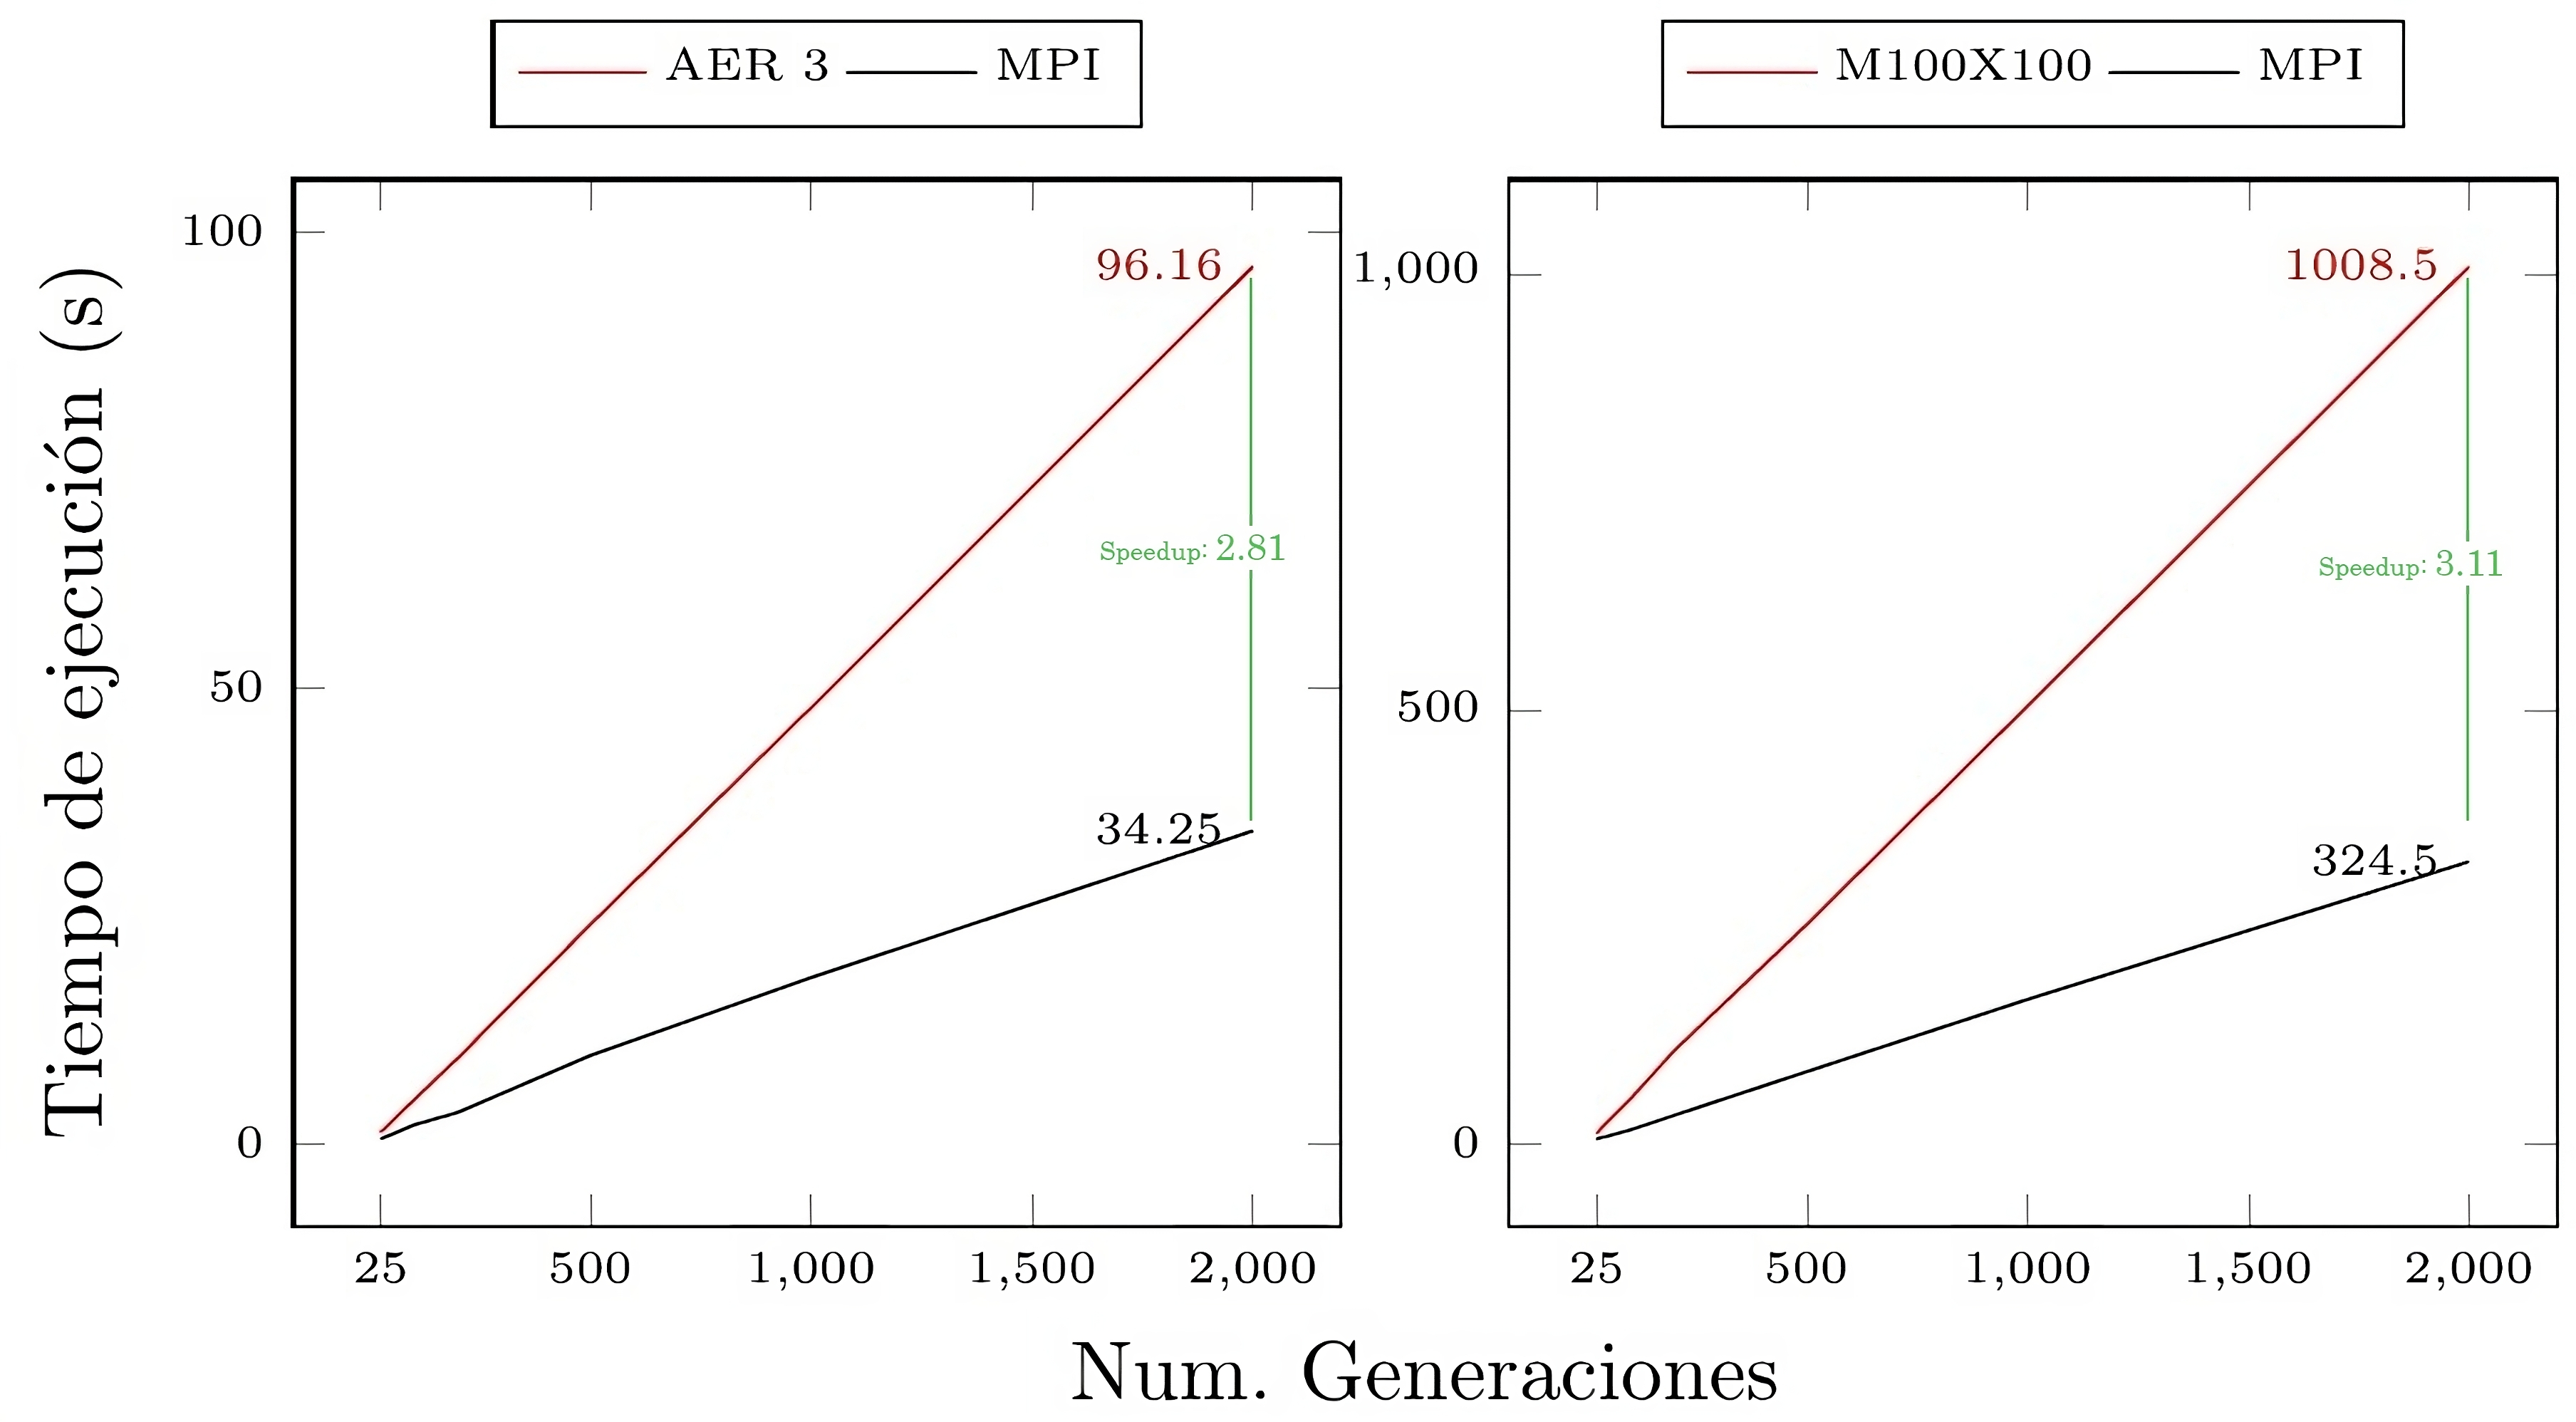
\includegraphics[width=0.7\textwidth]{images/chapter_4/pev_mpi1}
	\caption{Tiempo de ejecución del algoritmo básico Jerarquíco Aglomerativo}
	\label{fig:MPI1.2 - Dividir Poblacion + Speedup}
\end{figure}

% CODIGO DE LA IMAGEN DE ARRIBA
%\begin{figure}[h!]
%	\centering
%	\begin{tikzpicture}
%		\begin{groupplot}[group style={
%				group size=2 by 1, % Adjust group size (2 plots horizontally)
%				horizontal sep=0.78cm, % Adjust horizontal separation between plots
%				vertical sep=0.5cm}, % Adjust vertical separation between plots
%			width=0.40\textwidth, height=0.40\textwidth, % Adjust size as needed		
%			tick label style={font=\tiny} % Adjust font size of tick labels	
%			]
%			
%			% First plot
%			\nextgroupplot[title={}, ylabel=Tiempo de ejecución (s),
%			legend style={at={(0.5,1.05)},anchor=south,legend columns=-1},
%			xtick={25, 500, 1000, 1500, 2000}]
%			\addplot [mark=none, color=red] table [x index=0, y index=1, col sep=space] {files/pev_1_2mpi.txt};
%			\addplot [mark=none, color=black] table [x index=0, y index=2, col sep=space] {files/pev_1_2mpi.txt};			
%			\addlegendentry{\tiny AER 3}
%			\addlegendentry{\tiny MPI}
%			
%			% Add value labels
%			\node at (axis cs:2000,96.16) [text=red,left] {\tiny 96.16};
%			\node at (axis cs:2000,34.25) [text=black,left] {\tiny 34.25};
%			
%			% Second plot
%			\nextgroupplot[title={},
%			legend style={at={(0.5,1.05)},anchor=south,legend columns=-1},
%			xtick={25, 500, 1000, 1500, 2000}]
%			\addplot [mark=none, color=red] table [x index=0, y index=3, col sep=space] {files/pev_1_2mpi.txt};			
%			\addplot [mark=none, color=black] table [x index=0, y index=4, col sep=space] {files/pev_1_2mpi.txt};			
%			\addlegendentry{\tiny M100X100}
%			\addlegendentry{\tiny MPI}
%			
%			% Add value labels
%			\node at (axis cs:2000,1008.51) [text=red,left] {\tiny 1008.5};
%			\node at (axis cs:2000,324.52) [text=black,left]{\tiny 324.5};
%			
%		\end{groupplot}	
%		
%		% Common x-axis label
%		\node at ($(group c1r1.south)!0.5!(group c2r1.south) + (0,-0.4cm)$) [below] {Num. Generaciones};
%		
%	\end{tikzpicture}
%	\caption{MPI1.2 - Dividir Poblacion}
%\end{figure}


Como se comentó antes, al aumentar los tamaños se consiguen mejores resultados. Con estas características, la ejecución se aumenta al punto de ser buena opción aplicar esta mejora.

\underline{Mejora 3, PipeLine}

El método de pipeline varía para cada problema. Los individuos binarios no mejoran mucho la ejecución, al tener muchos datos que enviar. Sin embargo los problemas con individuos reales o árboles si se pueden optimizar. La evaluación es el método que más tarda en estos dos problemas, por lo que repartir la carga de trabajo con más procesos reduce el tiempo de ejecución.


\begin{figure}[h!]
	\centering
	\begin{tikzpicture}
		\begin{groupplot}[group style={
				group size=3 by 1,
				horizontal sep=0.78cm, % Adjust horizontal separation between plots
				vertical sep=0.5cm}, % Adjust vertical separation between plots
			width=0.40\textwidth, height=0.40\textwidth, % Adjust size as needed		
			tick label style={font=\tiny} % Adjust font size of tick labels	
			]
			
			% First plot
			\nextgroupplot[title={}, ylabel=Tiempo de ejecución (s),
			legend pos=north west,
			xtick={25, 500, 1000, 1500, 2000}]
			\addplot [mark=none, color=red] table [x index=0, y index=1, col sep=space] {files/pev_3mpi.txt};
			\addplot [mark=none, color=darkgreen] table [x index=0, y index=2, col sep=space] {files/pev_3mpi.txt};
			\addplot [mark=none, color=blue] table [x index=0, y index=3, col sep=space] {files/pev_3mpi.txt};							
			\addlegendentry{\tiny P10}
			\addlegendentry{\tiny MPI(4)}
			\addlegendentry{\tiny MPI(7)}
			
			
			% Second plot
			\nextgroupplot[title={},
			legend pos=north west,
			xtick={25, 500, 1000, 1500, 2000}]
			\addplot [mark=none, color=red] table [x index=0, y index=4, col sep=space] {files/pev_3mpi.txt};			
			\addplot [mark=none, color=darkgreen] table [x index=0, y index=5, col sep=space] {files/pev_3mpi.txt};
			\addplot [mark=none, color=blue] table [x index=0, y index=6, col sep=space] {files/pev_3mpi.txt};	
			\addlegendentry{\tiny AER3}
			\addlegendentry{\tiny MPI(6)}
			\addlegendentry{\tiny MPI(10)}
			
		\end{groupplot}	
		
		% Common x-axis label
		\node at ($(group c1r1.south)!0.5!(group c2r1.south) + (0,-0.4cm)$) [below] {Num. Generaciones};
		
	\end{tikzpicture}
	\caption{MPI3 - PipeLine}
\end{figure}

Para los individuos binarios, funciona algo mejor que la mejora anterior, con el funcionamiento de pipeline no se pierde tanto tiempo con el paso de mensajes de individuos binarios, y aunque sea poco, se puede reducir el tiempo de ejecución. Al tener varias poblaciones ejecutándose al mismo tiempo no se puede tener una población muy grande. A partir de un tamaño de 1000 no se puede ejecutar con dos decimales de precisión. 500 para 10 decimales de precisión.


\begin{figure}[!h]
\begin{mdframed}[roundcorner=5pt]
	\textbf{Binarios}
	\vspace{-0.2cm}
	
	\begin{tcolorbox}[boxrule=0.5pt, fontupper=\small]
		\scriptsize		
		\color{darkgreen} 1. Cuatro procesos: \color{black}\\
		- Master se encarga de inicializar\\
		- Worker1: evaluación y selección, procesos que no tardan mucho en ejecutarse.\\
		- Worker2: cruce\\
		- Worker3: mutación\\
		
		\color{blue} 2. Siete procesos. \color{black}\\
		Se duplica el numero de workers en cada pipe.	
	\end{tcolorbox}
	
	\vspace{-0.5cm}
	\begin{flushleft}
		\textbf{Reales}
	\end{flushleft}
	\vspace{-0.7cm}
	
	\begin{tcolorbox}[boxrule=0.5pt, fontupper=\small]
		\scriptsize
		Solo aumenta el número de workers en el método de evaluación.\\
		\color{darkgreen} 1. Seis procesos: \color{black}\\
		- Master se encarga de inicializar\\
		- Worker [1, 4]: evaluación, función que más tarda\\
		- Worker 5:  selección, cruce y mutación\\	
		
		\color{blue} 2. Diez procesos. \color{black}\\
		 Se duplica el numero de workers en cada pipe.	
	\end{tcolorbox}
	
	\vspace{-0.5cm}
	\begin{flushleft}
		\textbf{Arboles}
	\end{flushleft}
	\vspace{-0.4cm}
	Es igual que la implementación de individuos reales, pues la evaluación es el método que más tarda.
		
	
	
\end{mdframed}
\end{figure}

Estos datos se calcularon teniendo en cuenta los tiempos de ejecución para cada método (tabla del principio). \\
1. Evaluación $\approx$ 400e-06s \\
2. Selección $\approx$ 8e-06\\
3. Cruce $\approx$ 40e-06\\
4. Mutación $\approx$ 10e-06\\
Al juntar los últimos tres métodos, tarda un tiempo aproximado de 58e-06. \\
6.9 veces más rápido que la evaluación. Por simplicidad, es mejor ejecutar potencias de dos procesos, para hacer una división equitativa

% TODO PEV CLUSTER

\color{blue} TODO CLUSTER

\color{black}
\newpage

\begin{flushleft}
	\textbf{Redes Neuronales}
\end{flushleft}

Red neuronal con capa oculta 1x5, una capa y cinco nodos.

\begin{figure}[!h]
	\centering
	\begin{tikzpicture}
		\begin{axis}[
			xlabel={Num. Repeticiones},
			ylabel={Tiempo de ejeución (s)},
			legend pos=north west,
			grid=major,
			width=\textwidth,
			height=0.45\textwidth
			]
			
			% Plot data from the file without markers, with different colors, and thicker lines
			\addplot [mark=none, color=red, line width=1.2pt] table [x index=0, y index=1, col sep=space] {files/redneu1.txt};
			\addplot [mark=none, color=darkgreen, line width=1.2pt] table [x index=0, y index=2, col sep=space] {files/redneu1.txt};
			\addplot [mark=none, color=black, line width=1.2pt] table [x index=0, y index=3, col sep=space] {files/redneu1.txt};
			
			% Add legends
			\addlegendentry{Secuencial}
			\addlegendentry{Síncrono}
			\addlegendentry{Asíncrono}
			
			
		\end{axis}
	\end{tikzpicture}
	\caption{MPI1 - Red Neuronal}
\end{figure}

Una vez implementado para una red neuronal pequeña, no reduce el tiempo de ejecución. En programación evolutiva, el flujo de mensajes es unidireccional, y no se pierde tanto tiempo entre mensajes. Este algoritmo tiene dos métodos en diferentes direcciones, provocando un \textbf{flujo bidireccional}, y la comunicación entre procesos se ralentiza. Usando mensajes \textbf{asíncronos}, permite a cada proceso ejecutar antes el cálculo de forward y cuando recibe los errores los actualiza. Reduce muy poco el tiempo comparándolo con la versión síncrona, pero empeora la predicción del modelo.
También hay que tener en cuenta que el flujo de mensajes hace que el modelo aprenda con valores desactualizados. Y dependiendo de la población puede haber un bucle en el cual aumenta y reduce los pesos, provocando un entrenamiento erróneo.

% TODO REDNEU 5X50

\color{blue} TODO PROBAR CON 5X50

\color{black}
\newpage

Para dividir la población de entrenamiento, aplicando la idea de fine-tuning, entre los procesos hay que tener mucho cuidado. La repartición de individuos es crucial para un correcto aprendizaje de la red. Si cada proceso tiene la misma población de entrenamiento, se reduce el tiempo de ejecución en relación al número de procesos ejecutados, pero no garantiza buenas predicciones, pues la media sería parecida. A no ser que cada proceso inicialmente tuviese pesos distintos, aunque no se podría garantizar un buen entrenamiento. Sin embargo dividiendo la población de manera eficiente se podría intentar provocar que cada proceso aprendiese unos ciertos intervalos, y con una red grande ciertos nodos se especializan en unos datos, y no se entrelazan los resultados, llegando a reducir el tiempo y entrenar correctamente.

\begin{figure}[!h]
	\centering
	\begin{tikzpicture}
		\begin{axis}[
			xlabel={Num. Repeticiones},
			ylabel={Tiempo de ejeución (s)},
			legend pos=north west,
			grid=major,
			width=\textwidth,
			height=0.45\textwidth
			]
			
			% Plot data from the file without markers, with different colors, and thicker lines
			\addplot [mark=none, color=red, line width=1.2pt] table [x index=0, y index=1, col sep=space] {files/redneu2.txt};
			\addplot [mark=none, color=darkgreen, line width=1.2pt] table [x index=0, y index=2, col sep=space] {files/redneu2.txt};
			\addplot [mark=none, color=black, line width=1.2pt] table [x index=0, y index=3, col sep=space] {files/redneu2.txt};
			
			% Add legends
			\addlegendentry{Secuencial}
			\addlegendentry{MPI(2)}
			\addlegendentry{MPI(4)}
			
			
		\end{axis}
	\end{tikzpicture}
	\caption{MPI2 - Red Neuronal Dividiendo entrenamiento}
\end{figure}

Esta prueba se ejecutó con 80 individuos en la población de entrenamiento, sobre una red neuronal con diez capas ocultas y diez nodos por capa (10x10). Si aumentamos o reducimos la población o la estructura de la red, el tiempo será proporcional.
Al dividir la fase de entrenamiento se puede alcanzar un speedup aproximado al ideal, pero lo difícil es encontrar los valores concretos de los hiper parámetros y la repartición del entrenamiento para tener una buena red neuronal que cumpla con el funcionamiento deseado. Para ello se puede realizar una búsqueda en paralelo comprobando los mejores resultados, tanto variando la tasa de aprendizaje como la repartición de los individuos con los cuales se entrena al modelo.

Para realizar la búsqueda de mejores hiper parámetros se ejecuta, con los mismos pesos, varias veces con diferentes valores, almacenando los mejores resultados y cuando se obtienen. Con cien repeticiones con un tamaño de población de ochenta individuos y una precisión de 0.01 se pueden comprobar los resultados en un intervalo de [0.01,0.20].


% TODO CENTRAR BIEN
\begin{figure}[!h]
	\centering
	
	
	\begin{subfigure}[t]{0.35\textwidth}
		\begin{tikzpicture}
			\begin{axis}[
				ybar,
				bar width=0.35cm,
				ylabel={Tiempo de ejecución (s)},
				xlabel={Capa Oculta},
				symbolic x coords={5x1, 10x2, 20x3},
				xtick=data,
				enlarge x limits=0.2,
				ymin=0,
				%legend style={at={(0.5,-0.15)}, anchor=north, legend columns=-1},
				legend pos={north west},
				area legend
				]
				
				\addplot+[ybar, pattern=vertical lines, draw=black] plot coordinates 
				{(5x1, 2.342097799992189) (10x2, 10.170772599987686) (20x3, 45.124263799982145)};
				\addplot+[ybar, pattern=grid, draw=black] plot coordinates 
				{(5x1, 0.6505134999752045) (10x2, 2.6451210000086576) (20x3, 12.60217950004153)};
				
				
				
				\legend{Secuencial, MPI(4)}
			\end{axis}
		\end{tikzpicture}
		\label{fig:redneubusqueda}
		\caption{Grafica + SpeedUp}
	\end{subfigure}
	\hfill
	\begin{subfigure}[t]{0.55\textwidth}
		\centering
		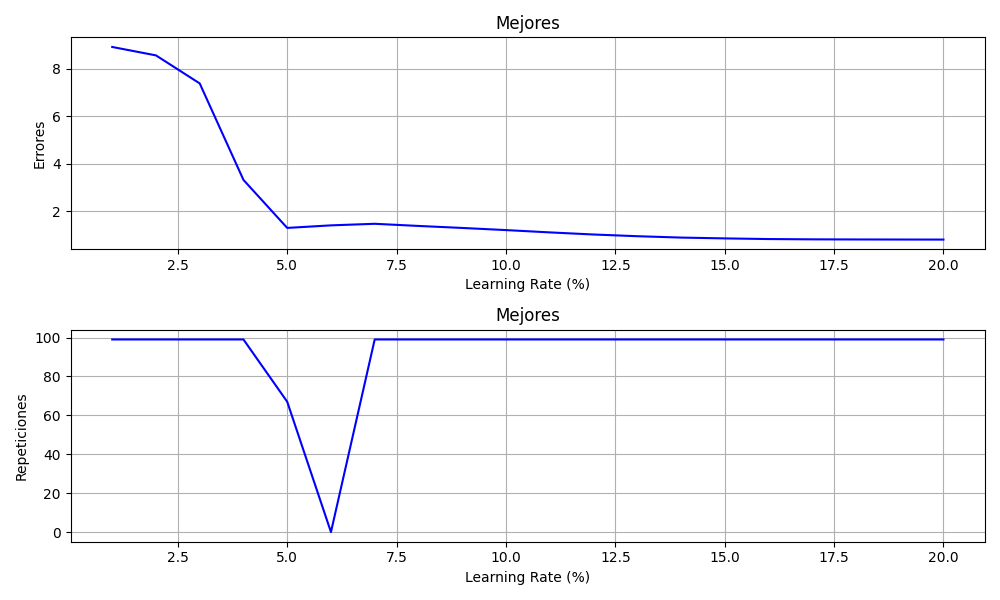
\includegraphics[width=0.8\textwidth,height=0.8\textwidth]{images/chapter_4/redneu_err}
		
		\caption{MPI - MergeSort}
		\label{fig:Errores}
	\end{subfigure}
	
	\caption{Mejoras MPI de las ordenaciones}
	\label{fig:Red Neuronal - Busqueda}
\end{figure}





Se ejecuta el algoritmo sobre varias configuraciones, en cada configuración siempre se utilizan los mismos pesos, para así comprobar cuales son los mejores hiper parámetros.

A la derecha se pueden ver los gráficos de la evolución, siendo el de arriba los errores cometidos en cada tasa de aprendizaje, y el de abajo cuando se obtienen menos errores.
